\documentclass{article}

\usepackage{amsmath, amsthm, amssymb, amsfonts}
\usepackage{thmtools}
\usepackage{graphicx}
\usepackage{setspace}
\usepackage{geometry}
\usepackage{float}
\usepackage{hyperref}
\usepackage[utf8]{inputenc}
\usepackage[english]{babel}
\usepackage{framed}
\usepackage[dvipsnames]{xcolor}
\usepackage{tcolorbox}

\colorlet{LightGray}{White!90!Periwinkle}
\colorlet{LightOrange}{Orange!15}
\colorlet{LightGreen}{Green!15}

\newcommand{\HRule}[1]{\rule{\linewidth}{#1}}

\declaretheoremstyle[name=Theorem,]{thmsty}
\declaretheorem[style=thmsty,numberwithin=section]{theorem}
\tcolorboxenvironment{theorem}{colback=LightGray}

\declaretheoremstyle[name=Proposition,]{prosty}
\declaretheorem[style=prosty,numberlike=theorem]{proposition}
\tcolorboxenvironment{proposition}{colback=LightOrange}

\declaretheoremstyle[name=Principle,]{prcpsty}
\declaretheorem[style=prcpsty,numberlike=theorem]{principle}
\tcolorboxenvironment{principle}{colback=LightGreen}

\theoremstyle{definition}
\newtheorem{definition}{Definition}[section]

\theoremstyle{remark}
\newtheorem*{remark}{Remark}

\newcommand{\argmin}{\mathop{\mathrm{argmin}}}
\newcommand{\argmax}{\mathop{\mathrm{argmax}}}
\newcommand{\minimize}{\mathop{\mathrm{minimize}}}
\newcommand{\maximize}{\mathop{\mathrm{maximize}}}
\newcommand{\st}{\mathop{\mathrm{subject\,\,to}}}
\newcommand{\tab}[1][1cm]{\hspace*{#1}}
\newcommand{\pdr}{\partial}

\def\R{\mathbb{R}}
\def\E{\mathbb{E}}
\def\P{\mathbb{P}}
\def\S{\mathbb{S}}
\def\Cov{\mathrm{Cov}}
\def\Var{\mathrm{Var}}
\def\half{\frac{1}{2}}
\def\sign{\mathrm{sign}}
\def\supp{\mathrm{supp}}
\def\th{\mathrm{th}}
\def\tr{\mathrm{tr}}
\def\dim{\mathrm{dim}}
\def\dom{\mathrm{dom}}


\def\hwnum{3}


\setstretch{1.2}
\geometry{
    textheight=9in,
    textwidth=5.5in,
    top=1in,
    headheight=12pt,
    headsep=25pt,
    footskip=30pt
}

% ------------------------------------------------------------------------------

\begin{document}

% ------------------------------------------------------------------------------
% Cover Page and ToC
% ------------------------------------------------------------------------------

\title{ \normalsize \textsc{}
		\\ [2.0cm]
		\HRule{1.5pt} \\
		\LARGE \textbf{\uppercase{Subgradient Algorithm}
		%\HRule{2.0pt} \\ [0.6cm] \LARGE{Subtitle}
        \vspace*{10\baselineskip}}
		}
\date{}
\author{\textbf{Author} \\ 
		Vinitra Muralikrishnan \\
		11th March, 2024}

\maketitle
\newpage

\tableofcontents
\newpage

% ------------------------------------------------------------------------------

\section{Overview}

\begin{definition}
    This is an algorithm to minimize a non-differentiable function
\end{definition}

It applies on:
\begin{itemize}
    \item non differentiable $f$
    \item step lengths or sizes are not searched by backtracking line search. They are fixed beforehand
    \item Unlike ordinary gradient descent methods, subgradient method is not a descent method. The function
    value can increase or decrease
\end{itemize}

\begin{definition}
    The subgradient of a convex function $f$ at $x$ is any $g \in \R^n$ s.t.
    $$f(y) \geq f(x) + g^T(y - x),\ \forall y$$
\end{definition}
The above definition stands for:
\begin{itemize}
    \item always exists for convex $f$
    \item for $f$ differentiable at $x$, then $g = \nabla f(x)$
    \item difficut to determine all subgradients at a point
    \item Also applicable for non-convex $f$
\end{itemize}
First order global underestimator:\\
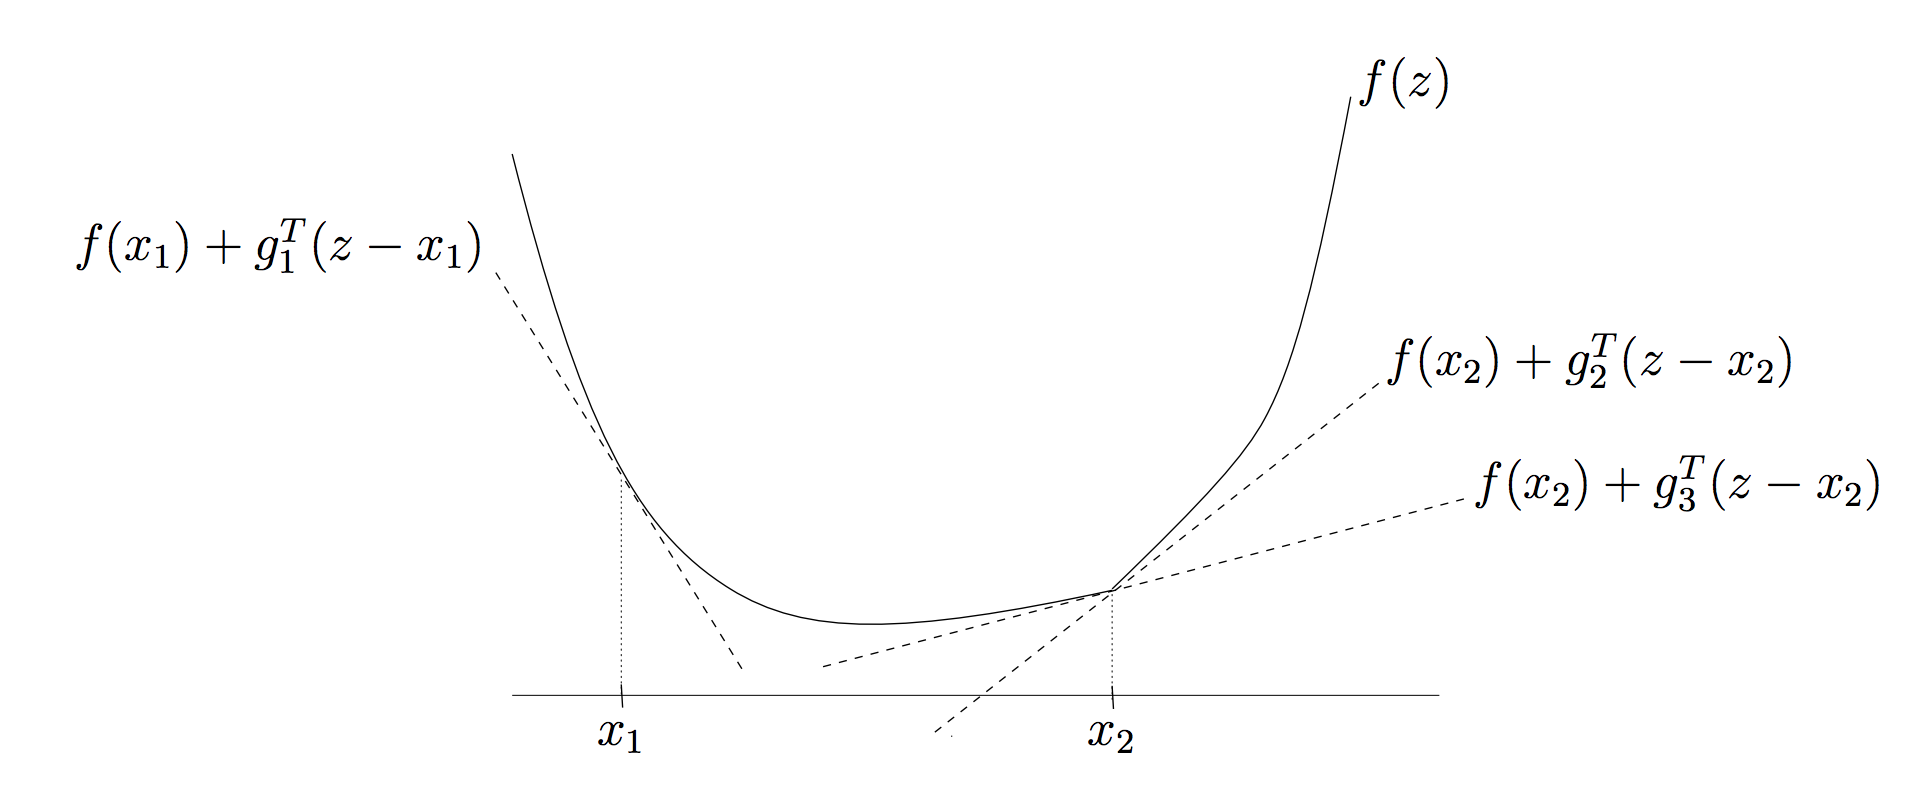
\includegraphics[width=5in]{img/subgradients.png}

\begin{remark}
    max of 2 functions $f_1, f_2$ is non-convex whether or not they are
    convex
\end{remark}

\begin{definition}
    The subdifferential is the set of all subgrdients of a convex $f$ at $x$\\
    $$\pdr f(x) = \{g \in \R^n: g \text{ is a subgradient of } f \text{ at } x\}$$
\end{definition}
The above definition implies:
\begin{itemize}
    \item non empty convex $f$
    \item $\pdr f(x)$ is closed and convex, even for non convex f
    \item $f$ is differentiable at $x \Leftrightarrow \pdr f(x) = \{\nabla f(x)\}$
\end{itemize}
\begin{remark}
    Subdifferential is a set while subgradient of a point is a vector.
\end{remark}
\begin{remark}
    Subgradient algorithm is not a descent method. It can move in any direction and keeps track of the best
    value so far.
\end{remark}
\section{References}
\begin{itemize}
    \item \href{https://see.stanford.edu/materials/lsocoee364b/01-subgradients_notes.pdf}{Stanford Lecture Notes}
\end{itemize}
%\begin{theorem}
    %This is a theorem.
%\end{theorem}

%\begin{proposition}
    %This is a proposition.
%\end{proposition}

%\begin{principle}
    %This is a principle.
%\end{principle}

%% Maybe I need to add one more part: Examples.
%% Set style and colour later.

%\subsection{Pictures}

%\begin{figure}[htbp]
    %\center
    %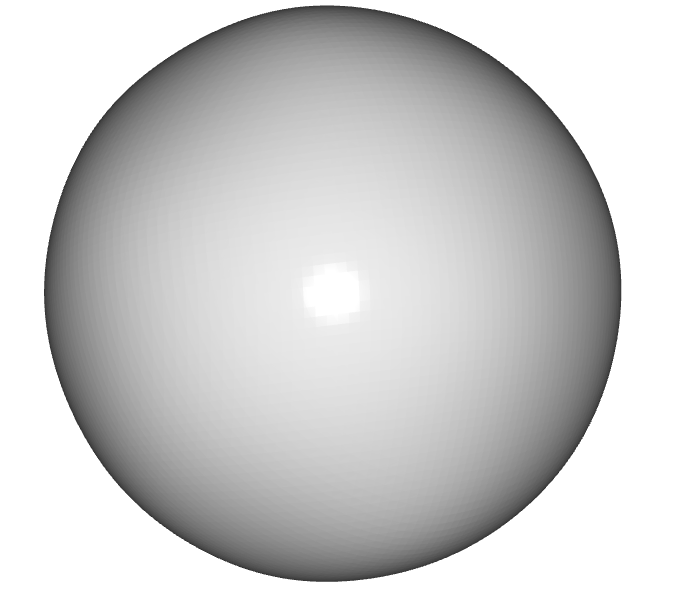
\includegraphics[scale=0.06]{img/photo.png}
    %\caption{Sydney, NSW}
%\end{figure}

%\subsection{Citation}

%This is a citation\cite{Eg}.

%\newpage

% ------------------------------------------------------------------------------
% Reference and Cited Works
% ------------------------------------------------------------------------------

\bibliographystyle{IEEEtran}
\bibliography{References.bib}

% ------------------------------------------------------------------------------

\end{document}
